

\documentclass[bigger]{beamer}

\usepackage{style}
\usepackage{subfiles}


\title[GRIN] %optional
{A modern look at GRIN}

\subtitle{an optimizing functional language back end}

\author[P. Podlovics, Cs. Hruska, Andor Pénzes ] % (optional, for multiple authors)
{Podlovics P\'eter - Hruska Csaba, Kaposi Ambrus}

\institute[ELTE] % (optional)
{
	Eötvös Loránd Tudom\'anyegyetem \\ Budapest
}

\date{EFOP \\ 2019/20/2} % (optional)



\begin{document}
	
{
	\usebackgroundtemplate{
\includegraphics[width=\paperwidth]{title.jpg}}%
	\frame{\vspace{15mm}\titlepage}
}

\begin{frame}
	\frametitle{Tartalom}
	\tableofcontents
\end{frame}


\section{GRIN \'attekint\'es}


\begin{frame}
\frametitle{Graph Reduction Intermediate Notation}

\begin{figure}[h]
	\centering
	\begin{adjustbox}{scale = 1.4}
		\tikzset{every loop/.style={-{Stealth[scale=1.5]}}}
		
		\begin{tikzpicture}[ node distance = 1.5cm and 1.5cm
		, on grid 
		, loop/.append style={-triangle 60}
		]
		
		\node [draw=black] (haskell)    									{Haskell};
		\node [draw=black] (idris)   [left  =of haskell]  {Idris};
		\node [draw=black] (agda)    [right =of haskell]  {Agda};
		\node [draw=black] (grin)    [below =of haskell]  {GRIN};
		\node [draw=black] (mc)      [below =of grin]     {LLVM};
		
		\path[-{Stealth[scale=1.5]}] 
		(idris) edge [] (grin)
		(haskell) edge [] (grin)
		(agda) edge [] (grin)
		(grin) edge [] (mc);
		
		
		\end{tikzpicture}
	\end{adjustbox}
	\label{grin-backend}
\end{figure}
\end{frame}


\begin{frame}[fragile]
\frametitle{Front end kód}

\begin{minipage}{0.35\textwidth}
	
	\begin{haskellcode}
		main = sum (upto 0 10)
		
		upto n m
		  | n > m = []
		  | otherwise = n : upto (n+1) m
		
		sum []     = 0
		sum (x:xs) = x + sum xs
	\end{haskellcode}
\end{minipage}

\end{frame}


\begin{frame}[fragile]
\frametitle{GRIN kód}

\begin{minipage}{0.4\textwidth}
	
	\begin{haskellcode}
		grinMain = 
		  t1 <- store (CInt 1)
		  t2 <- store (CInt 10)
		  t3 <- store (Fupto t1 t2)
		  t4 <- store (Fsum t3)
		  (CInt r) <- eval t4
		  _prim_int_print r
	\end{haskellcode}
\end{minipage}
\hfill
\begin{minipage}{0.48\textwidth}
	\vspace{1cm}
	\begin{haskellcode}
		eval p = 
		  v <- fetch p
		  case v of
		    (CInt n)     -> pure v
		    (CNil)       -> pure v
		    (CCons y ys) -> pure v
		    (Fupto a b) -> 
		      zs <- upto a b
		      update p zs
		      pure zs
		    (Fsum c) -> 
		      s <- sum c
		      update p s
		      pure s
	\end{haskellcode}
\end{minipage}


\end{frame}

\section{Datalog \'attekint\'es}

\begin{frame}
\frametitle{Logikai programozás}

  \begin{align*}
  	\scalebox{1.5}{$c \leftarrow p_1 \land p_2 \land \dots \land p_n$}
  \end{align*}

\end{frame}

\begin{frame}
\frametitle{A GRIN nyelv Datalog modellje (részlet)}
      \begin{mathpar}
  	\EmissionRule{\Store{p}{n}}
  	{\pilcode{p <- store n}}
  	{ER-Store}
  	\and
  	\EmissionRule{\Fetch{n}{p}}
  	{\pilcode{n <- fetch p}}
  	{ER-Fetch}
  	\and
  	\EmissionRule{\Update{x}{p}{n}}
  	{\pilcode{x <- update p n}}
  	{ER-Update}
  	\and
  	\EmissionRule{\LitAssign{k}{\tau(lit)}{lit}}
  	{\pilcode{k <- pure <lit>}}
  	{ER-Lit}
  	\and
  	\EmissionRule{\Move{y}{x}}
  	{\pilcode{y <- pure x}}
  	{ER-Move}
  \end{mathpar}
\end{frame}

\begin{frame}
\frametitle{Egyszerű points-to elemzés Datalog-ban}
\begin{mathpar}
	\InferRule{\Store{p}{n}}
	{\Heap{p}{n}}
	{H-Store}
	\and
	\InferRule{\Update{\any}{p}{n}}
	{\Heap{p}{n}}
	{H-Update'}
\end{mathpar}
\end{frame}


\section{Strukturális holt-kód eltávolítás}

\begin{frame}[fragile]
	\frametitle{Idris példa}
	
	\begin{center}
		\begin{minipage}{0.40\textwidth}
			\begin{haskellcode}
            length : List a -> Int
            length Nil = 0
            length (Cons x xs) 
              = 1 + length xs
			\end{haskellcode}
		\end{minipage}
		$\xRightarrow{\text{DDE}}$
		\pause
		\begin{minipage}{0.40\textwidth}
			\begin{haskellcode}
			length : List a -> Int
			length Nil = 0
			length (Cons xs) 
			  = 1 + length xs
			\end{haskellcode}
		\end{minipage}
	\end{center}
	
\end{frame}

\begin{frame}[fragile]
\frametitle{A generált GRIN kód}

  \begin{center}
  	\begin{minipage}{0.40\textwidth}
  		\begin{haskellcode}
		length : List a -> Int
		length Nil = 0
		length (Cons x xs) 
		  = 1 + length xs
  		\end{haskellcode}
  	\end{minipage}
  	\hfill
  	\pause
  	\begin{minipage}{0.50\textwidth}
  		\begin{overprint}
  		\onslide<2>
 		\begin{haskellcode}
		length p =
		  xs <- fetch p
		  case xs of
		    (Cons y ys) ->
		      l1 <- length ys
		      l2 <- int_add l1 1
		      pure l2
		    (Nil) ->
		      pure 0
  		\end{haskellcode}
  		\onslide<3>
  		\begin{haskellcode}
		length p =
		  xs <- fetch p
		  r <- case xs of
		    (Cons y ys) @ alt1 ->
		      l1 <- length ys
		      k1 <- pure 1
		      l2 <- int_add l1 k1
		      pure l2
		    (Nil) @ alt2 ->
		      k0 <- pure 0
		      pure k0
		  pure r
  		\end{haskellcode}
  	\end{overprint}
  	\end{minipage}
  \end{center}

\end{frame}

\begin{frame}[fragile]
\frametitle{A GRIN program Datalog reprezentációja}
\begin{center}
	\begin{minipage}{0.50\textwidth}
		\begin{haskellcode}
		length p =
		  xs <- fetch p
		  r <- case xs of
		    (Cons y ys) @ alt1 ->
		      l1 <- length ys
		      k1 <- pure 1
		      l2 <- int_add l1 k1
		      pure l2
		    (Nil) @ alt2 ->
		      k0 <- pure 0
		      pure k0
		  pure r
		\end{haskellcode}
	\end{minipage}
	\hfill 
	\pause
	\begin{minipage}{0.425\textwidth}
		\vspace{0.5cm}
		\begin{haskellcode}
        FunParam(length,0,p)
        Fetch(xs,p)
        Case(r,xs)
        Alt(r,alt1,CCons)
        AltParam(r,CCons,0,y)
        AltParam(r,CCons,1,ys)
        Call(l1,length)
        CallArgument(l1,0,ys)
        LitAssign(k1,Int,1)
        Call(l2,int_add)
        CallArgument(l2,0,l1)
        CallArgument(l2,1,k1)
        ReturnValue(alt1,l2)
		\end{haskellcode}
		\dots
	\end{minipage}
\end{center}
\end{frame}

\begin{frame}[fragile]
	\frametitle{Az élőségi elemzés eredménye (részlet)}
	
	\begin{center}
		\begin{minipage}{0.50\textwidth}
			\begin{minipage}{0.50\textwidth}
			\begin{overprint}
				\onslide<1>
				\begin{haskellcode}
				length p =
				  xs <- fetch p
				  r <- case xs of
				    (Cons y ys) @ alt1 ->
				      l1 <- length ys
				      k1 <- pure 1
				      l2 <- int_add l1 k1
				      pure l2
				    (Nil) @ alt2 ->
				      k0 <- pure 0
				      pure k0
				  pure r
				\end{haskellcode}
				\onslide<2>
				\begin{haskellcode}
					length p =
					  xs <- fetch p
					  r <- case xs of
					    (Cons y ys) @ alt1 ->
					       l1 <- length ys
					       k1 <- pure 1
					       l2 <- int_add l1 k1
					       pure l2
					     (Nil) @ alt2 ->
					       k0 <- pure 0
					       pure k0
					  pure r*
				\end{haskellcode}
				\onslide<3>
				\begin{haskellcode}
					length p =
					  xs <- fetch p
					  r <- case xs of
					    (Cons y ys) @ alt1 ->
					      l1 <- length ys
					      k1 <- pure 1
					      l2 <- int_add l1 k1
					      pure l2*
					    (Nil) @ alt2 ->
					      k0 <- pure 0
					      pure k0*
					  pure r*
			    \end{haskellcode}
                \onslide<4>
                \begin{haskellcode}
                length p =
                  xs <- fetch p
                  r <- case xs of
                    (Cons y ys) @ alt1 ->
                      l1 <- length ys
                      k1 <- pure 1
                      l2* <- int_add l1 k1
                      pure l2*
                    (Nil) @ alt2 ->
                      k0* <- pure 0
                      pure k0*
                  pure r*
                \end{haskellcode}
                \onslide<5>
                \begin{haskellcode}
                   length p =
                     xs <- fetch p
                     r <- case xs of
                       (Cons y ys) @ alt1 ->
                         l1* <- length ys
                         k1* <- pure 1
                         l2* <- int_add l1 k1
                         pure l2*
                       (Nil) @ alt2 ->
                         k0* <- pure 0
                         pure k0*
                     pure r*
                \end{haskellcode}
                \onslide<6>
                \begin{haskellcode}
                   length p =
                     xs* <- fetch p
                     r <- case xs of
                       (Cons y ys) @ alt1 ->
                         l1* <- length ys
                         k1* <- pure 1
                         l2* <- int_add l1 k1
                         pure l2*
                       (Nil) @ alt2 ->
                         k0* <- pure 0
                         pure k0*
                     pure r*
                \end{haskellcode}
                \onslide<7>
                \begin{haskellcode}
                   length p* =
                     xs* <- fetch p
                     r <- case xs of
                       (Cons y ys) @ alt1 ->
                         l1* <- length ys
                         k1* <- pure 1
                         l2* <- int_add l1 k1
                         pure l2*
                       (Nil) @ alt2 ->
                         k0* <- pure 0
                         pure k0*
                     pure r*
                \end{haskellcode}
                \onslide<8,9>
                \begin{haskellcode}
                   length p* =
                     xs* <- fetch p
                     r <- case xs of
                       (Cons y ys*) @ alt1 ->
                         l1* <- length ys
                         k1* <- pure 1
                         l2* <- int_add l1 k1
                         pure l2*
                       (Nil) @ alt2 ->
                         k0* <- pure 0
                         pure k0*
                     pure r*
                \end{haskellcode}
		    
			\end{overprint}
			\end{minipage}
		\end{minipage}
		\hfill
		\onslide<9>
		\begin{minipage}{0.4\textwidth}
			\begin{tcolorbox}[tab2,tabularx={l|r}]
				Var			  & Liveness \\
				\hline\hline
				\pilcode{p}   & $\top$ \\\hline
				\pilcode{y}   & $\bot$ \\\hline
				\pilcode{xs}  & $Nil[], Cons[\bot,\top]$ \\\hline
				\pilcode{ys}  & $\top$ \\\hline\hline
				\pilcode{l1}  & $\top$	\\\hline
				\pilcode{k1}  & $\top$ \\\hline
				\pilcode{l2}  & $\top$ \\\hline
				\pilcode{k0}  & $\top$ \\\hline
				\pilcode{r}   & $\top (feltetelezes)$	\\
			\end{tcolorbox}
		\end{minipage}
	\end{center}
	
\end{frame}


\section{M\'er\'esi eredm\'enyek}

\begin{frame}[fragile]
\frametitle{Környezet}

	\vspace{1.5cm}
	\begin{vfitemize}
		\item Kis Idris programok: \\
		\textit{Type-driven Development with Idris} - Edwin Brady
		\item Interpretált GRIN programok, és futtatott gépi kód is
		\item Fordítasi- és futásidejú mérések
	\end{vfitemize}

	\vspace{-0.5cm}
	\begin{figure}[H] 
		\centering
		\begin{adjustbox}{scale = 0.75}
			\subfile{idris-compilation-pipeline}
		\end{adjustbox}
	\end{figure}

\end{frame}



\begin{frame}[fragile]
\frametitle{Length - GRIN statisztikák}
	% real example
	
	\begin{figure}
		\hspace{-1cm}
		\begin{minipage}{0.45\textwidth}
			\resizebox{\width}{5.5cm}{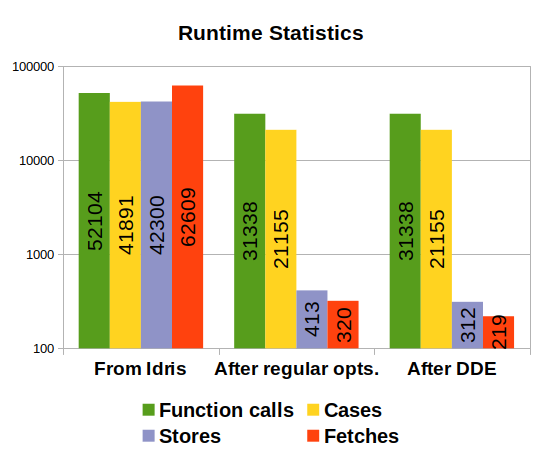
\includegraphics[scale=0.40]{length_rt.png}}
		\end{minipage}
		\hspace{1cm}
		\begin{minipage}{0.45\textwidth}
			\resizebox{\width}{5.5cm}{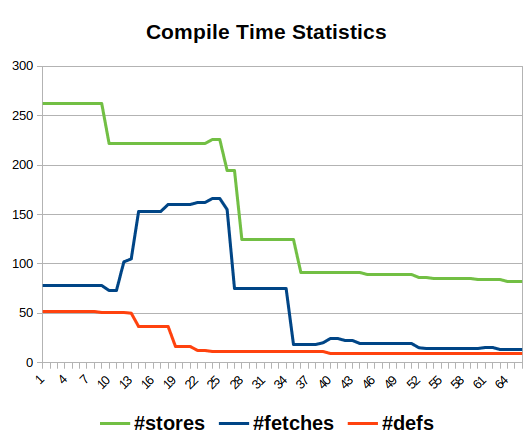
\includegraphics[scale=0.40]{length_ct.png}}
		\end{minipage}
	\end{figure}
	
\end{frame}

\begin{frame}[fragile]
\frametitle{Length - CPU bináris statisztikák}


    \hspace{-0.75cm}
	\begin{minipage}{1.075\textwidth}
		\begin{tcolorbox}[tab2,tabularx={l||r|r|r|r|r}]
			Stage                 & Size  & Inst. & Stores & Loads & Mem.    \\
			\hline\hline
			\pilcode{idris}       &     - & 2822725 & 366880 & 1064977 & 9440  \\\hline
			\pilcode{normal-O0}   & 23928 & 769588  & 212567 & 233305 & 674080  \\\hline
			\pilcode{normal-O3}   & 23928 & 550065  & 160252 & 170202 & 674080  \\\hline
			\pilcode{regular-opt} & 19832 & 257397  & 14848  & 45499  & 8200  \\\hline
			\pilcode{dde-O0}      & 15736 & 256062  & 14243  & 45083  & 5776  \\\hline	
			\pilcode{dde-O3}      & 15736 & 284970  & 33929  & 54555  & 5776  \\
		\end{tcolorbox}	
	\end{minipage}


\end{frame}

\begin{frame}[fragile]
\frametitle{Exact length - GRIN statisztikák}
	% no stores & no fetches! (Maybe transformed)
	\begin{figure}
		\hspace{-1cm}
		\begin{minipage}{0.45\textwidth}
			\resizebox{\width}{5.5cm}{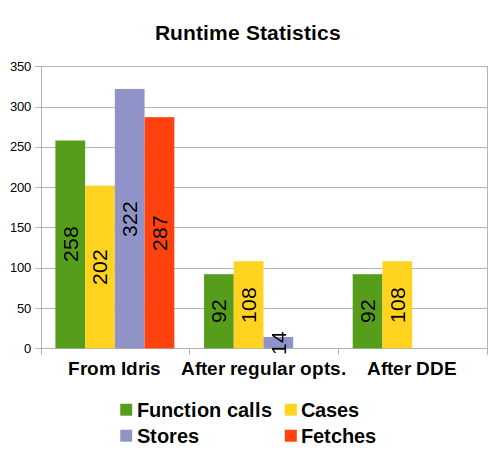
\includegraphics[scale=0.40]{exact_length_rt.png}}
		\end{minipage}
		\hspace{1cm}
		\begin{minipage}{0.45\textwidth}
			\resizebox{\width}{5.5cm}{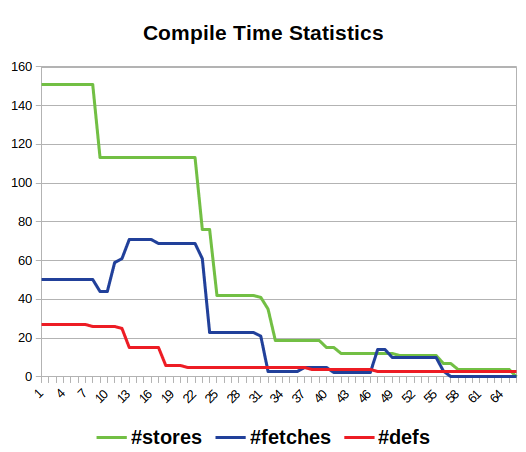
\includegraphics[scale=0.40]{exact_length_ct.png}}
		\end{minipage}
	\end{figure}
\end{frame}

\begin{frame}[fragile]
\frametitle{Exact length - CPU bináris statisztikák}

	\begin{minipage}{0.975\textwidth}
	\begin{tcolorbox}[tab2,tabularx={l||r|r|r|r|r}]
		Stage                 & Size  & Inst. & Stores & Loads & Mem.     \\
		\hline\hline
		\pilcode{idris}				&     - & 260393 & 23320 & 68334 & 1888  \\\hline
		\pilcode{normal-O0}   & 18800 & 188469 & 14852 & 46566 & 4112  \\\hline
		\pilcode{normal-O3}   & 14704 & 187380 & 14621 & 46233 & 4112  \\\hline
		\pilcode{regular-opt} & 10608 & 183560 & 13462 & 45214 & 112  \\\hline
		\pilcode{dde-O0}      & 10608 & 183413 & 13431 & 45189 & 0  \\\hline
		\pilcode{dde-O3}      & 10608 & 183322 & 13430 & 44226 & 0  \\
	\end{tcolorbox}	
\end{minipage}

\end{frame}

\section*{\"Osszefoglal\'o}

\begin{frame}[fragile]
\frametitle{\"Osszefoglal\'o}
	\begin{vfitemize}
		\item Újítasok:
			\begin{itemize}
				\item új szintaxis
				\item Datalog modell, Datalog elemzések
				\item strukturális holt-kód eltávolítás
			\end{itemize}
		\item Eredmények:
		\begin{itemize}
            \item a strukturális holt-kód eltávolítas képes jelentősen csökkenteni a bináris méretét
			\item a rendszer jól működik függőtípusos nyelvekre is
			\item az optimalizált GRIN kód jelentősen hatékonyabb
			\item a GRIN optimalizációk ortogonálisak az LLVM optimalizációkra
		\end{itemize}
	\end{vfitemize}
\end{frame}


{
	\usebackgroundtemplate{
\includegraphics[width=\paperwidth]{title.jpg}}%
	\begin{frame}{}
	
	\bigskip\bigskip\bigskip
	
	{\bf\Huge\color{white} KÖSZÖNÖM}

	
	\bigskip
	
	{\bf\Huge\color{white} A FIGYELMET!}
	
\end{frame}
}

% Q&A

\end{document}

